\let\negmedspace\undefined
\let\negthickspace\undefined
\documentclass[journal]{IEEEtran}
\usepackage[a5paper, margin=10mm, onecolumn]{geometry}
\usepackage{lmodern} % Ensure lmodern is loaded for pdflatex
\usepackage{tfrupee} % Include tfrupee package

\setlength{\headheight}{1cm} % Set the height of the header box
\setlength{\headsep}{0mm}     % Set the distance between the header box and the top of the text

\usepackage{gvv-book}
\usepackage{gvv}
\usepackage{cite}
\usepackage{amsmath,amssymb,amsfonts,amsthm}
\usepackage{algorithmic}
\usepackage{graphicx}
\graphicspath{{./figs/}}
\usepackage{textcomp}
\usepackage{xcolor}
\usepackage{txfonts}
\usepackage{listings}
\usepackage{enumitem}
\usepackage{mathtools}
\usepackage{gensymb}
\usepackage{comment}
\usepackage[breaklinks=true]{hyperref}
\usepackage{tkz-euclide} 
\usepackage{listings}
\usepackage{gvv}                                        
\def\inputGnumericTable{}                                 
\usepackage[latin1]{inputenc}                                
\usepackage{color}                                            
\usepackage{array}                                            
\usepackage{longtable}                                       
\usepackage{calc}                                             
\usepackage{multirow}                                         
\usepackage{hhline}                                           
\usepackage{ifthen}                                           
\usepackage{lscape}
\usepackage{circuitikz}
\tikzstyle{block} = [rectangle, draw, fill=blue!20, 
text width=4em, text centered, rounded corners, minimum height=3em]
\tikzstyle{sum} = [draw, fill=blue!10, circle, minimum size=1cm, node distance=1.5cm]
\tikzstyle{input} = [coordinate]
\tikzstyle{output} = [coordinate]


\begin{document}
	
	\bibliographystyle{IEEEtran}
	\vspace{3cm}
	
	\title{2.4.29}
	\author{EE25BTECH11042 - Nipun Dasari}
	\maketitle
	% \newpage
	% \bigskip
	{\let\newpage\relax\maketitle}
	
	\renewcommand{\thefigure}{\theenumi}
	\renewcommand{\thetable}{\theenumi}
	\setlength{\intextsep}{10pt} % Space between text and floats
	
	
	\numberwithin{equation}{enumi}
	\numberwithin{figure}{enumi}
	\renewcommand{\thetable}{\theenumi}
	
	\textbf{Question}:\\
	The points $\vec{A}\brak{2, 9}$, $\vec{B}\brak{a, 5}$ and $\vec{C}\brak{5, 5}$ are the vertices of a triangle $\vec{ABC}$ right angled
	at $\vec{B}$. Find the values of a and hence the area of $\Delta\vec{ABC}$. \\ 
	\solution \\
	
	Given the points A, B and C, also consider $\vec{c}$ to be vector opposite to side AB and $\vec{b}$, $\vec{a}$ similarly
	
	\begin{align}
		\vec{A} = \begin{myvec}{2\\9} \end{myvec} , \vec{B} = \begin{myvec}{a\\5} \end{myvec}, \vec{C} = \begin{myvec}{5\\5} \end{myvec}
	\end{align}
	Since the sides c and a are perpendicular their inner product will be 0\\
	Take the inner product of $\vec{c}$ and $\vec{a}$\\
	Vector $\vec{c}$:
	\begin{align}
		\vec{c} = \vec{A}-\vec{B} = \begin{myvec}{2 -a\\9 - 5} \end{myvec} = \begin{myvec}{2 -a\\4} \end{myvec}
	\end{align}
	Vector $\vec{a}$:
	\begin{align}
		\vec{a} = \vec{B}-\vec{C} = \begin{myvec}{a - 5\\5 - 5} \end{myvec} = \begin{myvec}{a - 5 \\0} \end{myvec}
	\end{align}
	Orthogonality $\implies$ matrix product is zero :
	\begin{align}
	\vec{c}^T\vec{a} = \begin{myvec}{2 -a & 4} \end{myvec}\begin{myvec}{a - 5 \\0} \end{myvec} = \brak{2-a}\brak{a-5} = 0
	\end{align}
	So \brak{2-a}\brak{5-a} = 0 $\implies$ $a = 2$ or $a = 5$.\\
	$a = 5$ make $\vec{B}$=$\vec{C}$. $\therefore a =2$  \\
	We can compute area using cross product formula
	\begin{align}
		\Delta = \frac{1}{2}\norm{\vec{c}\times\vec{a}} \label{eq:0.5}
	\end{align}
	The general cross product of two vectors is defined as:
	\begin{align}
		\vec{A}\times\vec{B} = \begin{myvec}{|\vec{A}_{23} & \vec{B}_{23}|\\|\vec{A}_{31} & \vec{B}_{31}|\\|\vec{A}_{12} & \vec{B}_{12}|} \end{myvec} \label{0.6}
	\end{align}
	 The vectors in 3-D space look like
	 \begin{align}
	 	\vec{c} = \begin{myvec}{0\\4\\0} \end{myvec}
	 \end{align}
	 \begin{align}
	 	\vec{a} = \begin{myvec}{-3 \\0\\0} \end{myvec}
	 \end{align}
	\begin{align}
		\vec{c}_{31} \text{ } \vec{a}_{31}| = |\begin{mydet}{0 & 0\\ 0 & -3} \end{mydet} = 0
	\end{align}
	\begin{align}
	|\vec{c}_{23} \text{ } \vec{a}_{23}| = \begin{mydet}{4 & 0\\ 0 & 0} \end{mydet} = 0
	\end{align}
	\begin{align}
	|\vec{c}_{12} \text{ } \vec{a}_{12}| = \begin{mydet}{0 & 4\\ -3 & 0} \end{mydet} = 12
	\end{align}
	By \eqref{0.6}:
	\begin{align}
		\vec{c}\times\vec{a} = \begin{myvec}{0 \\ 0 \\ 12} \end{myvec}
	\end{align}
	\begin{align}
		\norm{\vec{c}\times\vec{a}} = 12
	\end{align}
	
	
	
	Using \eqref{eq:0.5}
	\begin{align}
		\therefore	\Delta = \frac{1}{2}\norm{\vec{c}\times\vec{a}} = 6
	\end{align}
	Thus area of triangle is $6$\\

	
	\begin{figure}[H]
		\centering
		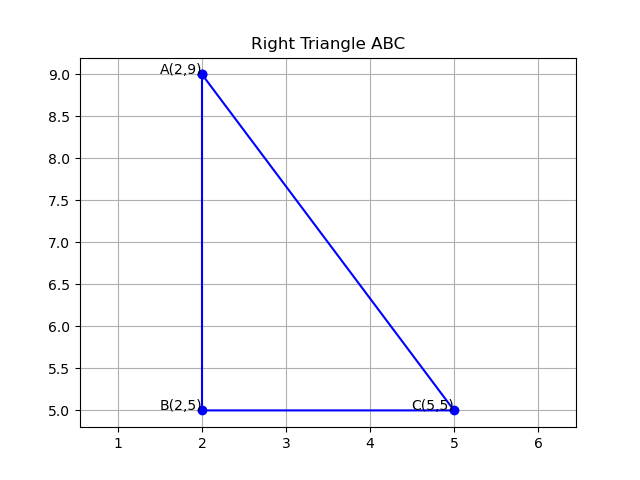
\includegraphics[width = 0.7\columnwidth]{Figure_1.png}
		\caption*{}
		\label{q3.1}
	\end{figure}
	
	\begin{figure}[H]
		\centering
		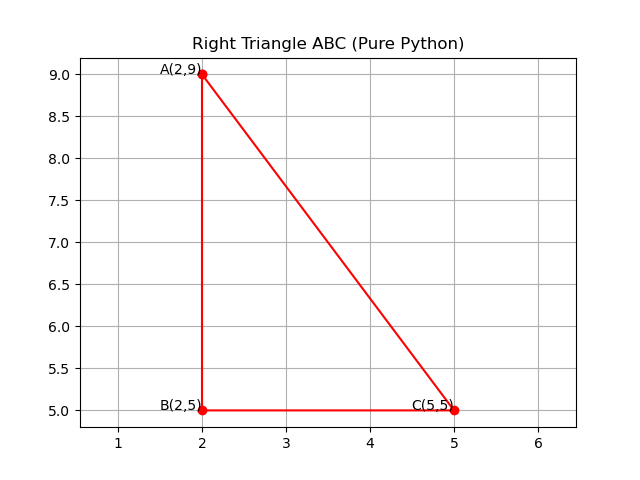
\includegraphics[width = 0.7\columnwidth]{Figure_2.png}
		\caption*{}
		\label{q3.2}
	\end{figure}
		
\end{document}


